%=============================================================================
% CS6886 -- System Engineering for Deep Learning, Assignment 2
% Single-column technical report
%=============================================================================
\documentclass[10pt,a4paper]{article}

\usepackage[a4paper,margin=0.95in]{geometry}
\usepackage[T1]{fontenc}
\usepackage{lmodern}
\usepackage{amsmath,amssymb}
\usepackage{graphicx}
\usepackage{booktabs}
\usepackage{colortbl}
\usepackage{xcolor}
\usepackage{caption}
\usepackage{microtype}
\usepackage[hidelinks]{hyperref}
\usepackage{titlesec}
\usepackage[htt]{hyphenat}  % permit line breaks inside long \texttt tokens
\sloppy
\emergencystretch=2em

\graphicspath{{figures/}}
\captionsetup{font=small,labelfont=bf,skip=4pt}
\setlength{\abovedisplayskip}{5pt}
\setlength{\belowdisplayskip}{5pt}
\setlength{\textfloatsep}{10pt}
\setlength{\parskip}{0pt}
\titlespacing*{\section}{0pt}{9pt plus 2pt minus 2pt}{5pt}
\titlespacing*{\subsection}{0pt}{7pt plus 1pt minus 1pt}{3pt}

% let floats pack more densely so figure-heavy pages do not leave gaps
\renewcommand{\topfraction}{0.92}
\renewcommand{\bottomfraction}{0.85}
\renewcommand{\textfraction}{0.07}
\renewcommand{\floatpagefraction}{0.75}
\setcounter{topnumber}{3}
\setcounter{bottomnumber}{2}
\setcounter{totalnumber}{5}

% ---------------------------------------------------------------------------
% results_tables.tex -- numeric tables; values from runs/*.json and runs/*.csv
% ---------------------------------------------------------------------------

% ---- Training recipe ------------------------------------------------------
\newcommand{\TableTraining}{%
\begin{table}[htbp]
\centering
\caption{Training configuration (\texttt{src/train.py}).}
\label{tab:train}
\small
\begin{tabular}{ll@{\hskip 3em}ll}
\toprule
Setting & Value & Setting & Value \\
\midrule
Optimiser     & SGD                & Batch size      & 128 \\
Momentum      & 0.9, Nesterov      & Epochs          & 180 \\
Weight decay  & $5\times10^{-4}$   & Label smoothing & 0.1 \\
Learning rate & 0.1                & Seed            & 42 \\
Warmup        & 5 epochs, linear   & GPU             & NVIDIA RTX A5000 \\
Scheduler     & cosine annealing   & Epoch time      & $\approx16$\,s \\
\bottomrule
\end{tabular}
\end{table}}

% ---- Per-class accuracy ---------------------------------------------------
\newcommand{\TablePerClass}{%
\begin{table}[htbp]
\centering
\caption{Per-class top-1 accuracy of the FP32 baseline (epoch-176 checkpoint)
over the 10{,}000-image CIFAR-10 test set.}
\label{tab:perclass}
\small
\begin{tabular}{lr@{\hskip 2.5em}lr@{\hskip 2.5em}lr}
\toprule
Class & Top-1 & Class & Top-1 & Class & Top-1 \\
\midrule
airplane   & 93.9\% & deer  & 93.5\% & ship  & 95.1\% \\
automobile & 96.7\% & dog   & 89.8\% & truck & 96.2\% \\
bird       & 91.3\% & frog  & 95.2\% & \textbf{Overall} & \textbf{93.18\%} \\
cat        & 85.6\% & horse & 94.5\% &       &  \\
\bottomrule
\end{tabular}
\end{table}}

% ---- Quantisation coverage ------------------------------------------------
\newcommand{\TableCoverage}{%
\begin{table}[htbp]
\centering
\caption{Quantised operators. All 53 Conv/Linear layers are quantised on both
the weight and the input-activation side.}
\label{tab:coverage}
\small
\begin{tabular}{lr@{\hskip 3em}lr}
\toprule
Layer type & Count & Layer type & Count \\
\midrule
Stem convolution ($3\times3$)     & 1  & Projection pointwise ($1\times1$) & 17 \\
Expansion pointwise ($1\times1$)  & 16 & Final convolution ($1\times1$)    & 1 \\
Depthwise ($3\times3$)            & 17 & Classifier (linear)               & 1 \\
\midrule
\multicolumn{3}{l}{Total quantised operators} & \textbf{53} \\
\bottomrule
\end{tabular}
\end{table}}

% ---- Uniform sweep --------------------------------------------------------
\newcommand{\TableUniform}{%
\begin{table}[htbp]
\centering
\caption{Uniform quantisation sweep (\texttt{runs/compression/}). Compression
ratios are tensor-level ratios for the quantised weights and for the
per-image activation memory.}
\label{tab:uniform}
\small
\begin{tabular}{lrrr}
\toprule
$b_W/b_A$ & Top-1 & Weight compression & Activation compression \\
\midrule
32/32 & 93.18\% & $1.00\times$  & $1.00\times$ \\
8/8   & 92.78\% & $4.00\times$  & $4.00\times$ \\
4/8   & 90.75\% & $8.00\times$  & $4.00\times$ \\
8/4   & 22.36\% & $4.00\times$  & $8.00\times$ \\
4/4   & 21.83\% & $8.00\times$  & $8.00\times$ \\
2/8   & 12.70\% & $16.00\times$ & $4.00\times$ \\
2/2   & 10.00\% & $16.00\times$ & $16.00\times$ \\
\bottomrule
\end{tabular}
\end{table}}

% ---- Mixed-precision / W&B sweep ------------------------------------------
\newcommand{\TableMixed}{%
\begin{table}[htbp]
\centering
\caption{Mixed-precision sweep logged to Weights \& Biases
(\texttt{runs/mixed\_precision/results.csv}). Compression is the whole-model
ratio recorded for each run; the selected configuration is highlighted.}
\label{tab:mixed}
\small
\begin{tabular}{lrr}
\toprule
Configuration & Top-1 accuracy & Compression \\
\midrule
\texttt{uniform\_w32a32} (baseline) & 93.18\% & $1.00\times$ \\
\texttt{uniform\_w8a8}              & 92.78\% & $3.74\times$ \\
\texttt{uniform\_w4a8}              & 90.75\% & $5.08\times$ \\
\texttt{uniform\_w4a4}              & 21.83\% & $6.91\times$ \\
\texttt{uniform\_w2a8}              & 12.70\% & $6.19\times$ \\
\texttt{hawq\_w8-4\_top75\_a8}      & 92.94\% & $4.14\times$ \\
\texttt{hawq\_w8-4\_top50\_a8}      & 92.69\% & $4.54\times$ \\
\rowcolor{black!8}
\textbf{\texttt{hawq\_w8-4\_top25\_a8}} & \textbf{92.28\%} & $\mathbf{5.05\times}$ \\
\texttt{hawq\_w8-4\_top10\_a8}      & 91.56\% & $5.07\times$ \\
\bottomrule
\end{tabular}
\end{table}}

% ---- Final storage accounting ---------------------------------------------
\newcommand{\TableFinal}{%
\begin{table}[htbp]
\centering
\caption{Final storage accounting for \texttt{hawq\_w8-4\_top25\_a8}. The total
model size includes 68{,}476\,B of scale metadata and 272{,}936\,B of retained
FP32 BatchNorm and bias tensors.}
\label{tab:final}
\small
\begin{tabular}{lrrr}
\toprule
Metric & FP32 & Compressed & Ratio \\
\midrule
Top-1 accuracy            & 93.18\%  & 92.28\%   & $-0.90$\,pt \\
Weight storage            & 8.402 MB & 1.069 MB  & $7.86\times$ \\
Activation memory / image & 6.194 MB & 1.549 MB  & $4.00\times$ \\
Total model size          & 8.662 MB & 1.395 MB  & $6.21\times$ \\
Average weight width      & 32 bits  & 4.07 bits & --- \\
\bottomrule
\end{tabular}
\end{table}}


\title{\vspace{-1.0cm}\textbf{MobileNet-v2 Compression on CIFAR-10:\\
Uniform Quantisation and Sensitivity-Guided Mixed Precision}}
\author{%
Name: \rule{4cm}{0.4pt} \qquad Roll Number: \rule{3cm}{0.4pt}\\[3pt]
GitHub: \rule{7cm}{0.4pt}\\[5pt]
CS6886 --- System Engineering for Deep Learning, Assignment 2\\
Indian Institute of Technology Madras}
\date{}

\begin{document}
\maketitle
\vspace{-0.9cm}

%=============================================================================
\section{Introduction}
%=============================================================================
The deployed cost of a convolutional network is dominated by storage rather than
arithmetic: parameters must be resident in memory, and activation tensors must be
buffered between operators. Reducing the numerical width of both is the most
direct lever on that footprint, and quantisation --- representing tensors on a
coarse integer grid instead of in 32-bit floating point --- is the standard
mechanism for doing so.

MobileNet-v2~\cite{sandler2018mobilenetv2} is a demanding subject for this
treatment: its inverted residual blocks expand a narrow bottleneck, apply a
depthwise $3\times3$ convolution and project back linearly, so the architecture is
already parameter-efficient and carries little redundancy to absorb quantisation
error. The evaluation workload is
CIFAR-10~\cite{krizhevsky2009cifar}: 50{,}000 training and 10{,}000 test images at
$32\times32$ resolution over ten classes.

Weight precision and activation precision are separate budgets, and this report
treats them as such throughout. Weights are quantised statically from the trained
tensors and are stored once; activations are quantised against ranges estimated
from calibration data and are re-materialised for every input. The experiments
below establish an FP32 baseline (Q1), sweep both widths uniformly to locate the
usable operating range (Q2), rank layers by second-order sensitivity to allocate
precision non-uniformly (Q3), and audit the resulting storage against the
uncompressed model (Q4).

%=============================================================================
\section{Experimental Setup}
%=============================================================================
\textbf{Dataset and preprocessing.} CIFAR-10 provides 50{,}000 training and
10{,}000 test images, $32\times32$ RGB, over ten classes. The training transform is
\texttt{RandomCrop(32, padding=4)} with reflect padding, then
\texttt{RandomHorizontalFlip(p=0.5)}, then \texttt{ToTensor} and
\texttt{Normalize}; the horizontal flip is applied with probability $p=0.5$. The
test transform is \texttt{ToTensor} and \texttt{Normalize} only, with no
stochastic operator, so evaluation is deterministic. Both splits use the
channel statistics of the training set,
$\mu = (0.4914, 0.4822, 0.4465)$ and $\sigma = (0.2470, 0.2435, 0.2616)$.

\textbf{Model.} The network is MobileNet-v2 with width multiplier $1.0$ on
$32\times32\times3$ inputs, reimplemented directly so that individual convolution
and BatchNorm modules stay addressable by name for the compression stage. The
published ImageNet schedule reduces resolution by $32\times$, which would drive a
$32\times32$ input below one pixel before the classifier, so the stem convolution
and the first expansion stage are set to stride 1. Total downsampling becomes
$8\times$ and the classifier sees a $4\times4\times1280$ feature map. The inverted-residual stages
$(t,c,n,s)$ are otherwise unchanged:
\[
\begin{array}{l}
(1,16,1,1)\;\; (6,24,2,1)\;\; (6,32,3,2)\;\; (6,64,4,2)\\[2pt]
(6,96,3,1)\;\; (6,160,3,2)\;\; (6,320,1,1),
\end{array}
\]
with $t$ the expansion factor, $c$ the output channels, $n$ the repeat count and
$s$ the stride of the first repeat. Activations are ReLU6, dropout is $0.2$
before the classifier, and the model has $2{,}236{,}682$ parameters. It is trained
from scratch: transferring $224\times224$ pretrained weights to $32\times32$
inputs would require the very stride and resolution changes that discard most of
the transferred benefit.

\textbf{Training.} Table~\ref{tab:train} lists the recipe. Optimisation uses SGD
with Nesterov momentum under a five-epoch linear warmup followed by cosine
annealing~\cite{loshchilov2017sgdr} to zero, with label smoothing $0.1$. A single
seed (42) is threaded through model initialisation, shuffling and worker seeding.

\TableTraining

%=============================================================================
\section{Q1 --- Baseline Model and Evaluation}
%=============================================================================

\subsection{Baseline Configuration}
The baseline is the model and recipe of the preceding section, trained for 180
epochs on one NVIDIA RTX A5000 at roughly 16\,s per epoch. The best test top-1
accuracy is \textbf{93.18\%}, recorded at \textbf{epoch 176}. At the final epoch
(180) the model reaches 98.70\% train and 93.04\% test accuracy; the $\sim$5.7\,pt
gap is mild overfitting, consistent with a 2.2M-parameter model trained for 180
epochs on 50{,}000 images under light augmentation.

The epoch-176 best checkpoint (\texttt{runs/baseline/best.pt}) is used unchanged
for every compression experiment in this report. No retraining, fine-tuning or
quantisation-aware training is performed at any later stage, so all subsequent
accuracy differences are attributable to quantisation alone.

\subsection{Data Augmentation}
Two stochastic transforms are applied at training time, resampled independently
at every epoch so a given image is seen under a different realisation each pass.
\texttt{RandomCrop(32, padding=4, reflect)} pads by four pixels per side and takes
a random $32\times32$ window, translating the object within the frame; reflect
padding avoids the black border that zero padding would introduce. \texttt{RandomHorizontalFlip(p=0.5)} mirrors the image with
probability $0.5$, which is label preserving for all ten CIFAR-10 classes,
whereas a vertical flip is not and is therefore excluded. Figure~\ref{fig:aug}
shows realisations of this pipeline.

\begin{figure}[htbp]
\centering
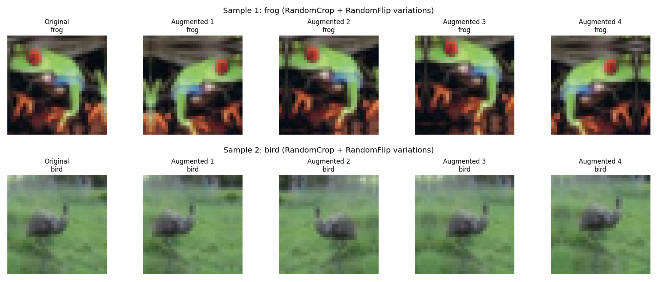
\includegraphics[width=0.88\textwidth]{augmentation_examples}
\caption{Training-time augmentation. Each row shows one original CIFAR-10 image
followed by four independent draws of \texttt{RandomCrop(32, padding=4, reflect)}
composed with \texttt{RandomHorizontalFlip(p=0.5)}. Images are displayed after
normalisation and inverse normalisation, so intensities match what the network
receives.}
\label{fig:aug}
\end{figure}

\subsection{Training and Test Curves}
Figures~\ref{fig:loss} and~\ref{fig:acc} plot the recorded per-epoch history over
the full 180-epoch schedule. Test accuracy oscillates through the
high-learning-rate middle of the schedule, with brief dips around epochs 45--80,
and smooths once cosine annealing brings the learning rate towards zero over the
final $\sim$30 epochs; the best test accuracy of 93.18\% at epoch 176 is marked in
Figure~\ref{fig:acc}. The reported losses include label smoothing, so neither
curve approaches zero at convergence.

\begin{figure}[htbp]
\centering
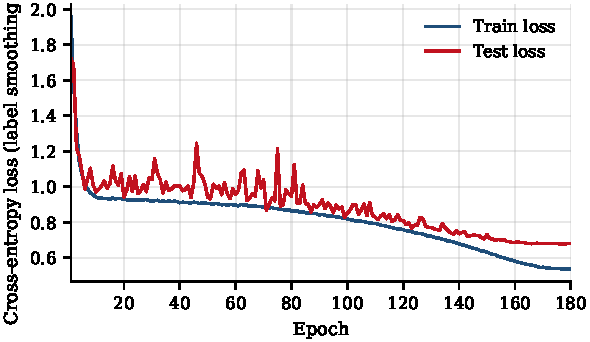
\includegraphics[width=0.58\textwidth]{loss_curve}
\caption{Training and test cross-entropy loss versus epoch, from
\texttt{runs/baseline/history.csv}. Losses include label smoothing $0.1$.}
\label{fig:loss}
\end{figure}

\begin{figure}[htbp]
\centering
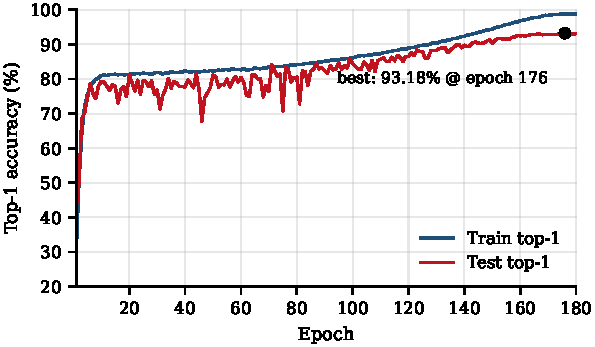
\includegraphics[width=0.58\textwidth]{accuracy_curve}
\caption{Training and test top-1 accuracy versus epoch. The marked point is the
best test accuracy, 93.18\% at epoch 176, which is the checkpoint used for all
compression experiments.}
\label{fig:acc}
\end{figure}

\subsection{Confusion Matrix}
Figure~\ref{fig:cm} shows the confusion matrix of the epoch-176 checkpoint over
all 10{,}000 test images, and Table~\ref{tab:perclass} gives the corresponding
per-class accuracies.

The error is concentrated in one symmetric pair rather than spread across the
matrix. Cat is the weakest class at 85.6\%, with 6.8\% of cats predicted as dogs;
dog is the second weakest at 89.8\%, with 6.2\% predicted as cats. Those two
cells alone account for roughly a fifth of the total classification error. The
remaining off-diagonal structure is an order of magnitude weaker and
semantically coherent --- the two vehicle classes exchange some mass, as do ship
and airplane --- which is the standard CIFAR-10 failure pattern and not specific
to this architecture.

\begin{figure}[htbp]
\centering
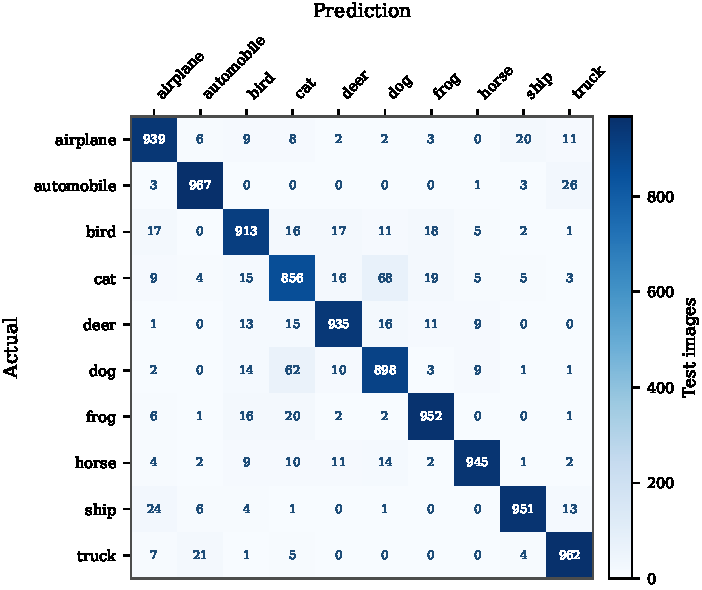
\includegraphics[width=0.80\textwidth]{confusion_matrix}
\caption{Confusion matrix of the FP32 baseline (epoch-176 checkpoint) over the
CIFAR-10 test set. Cells give test-image counts. Each class contributes exactly
1{,}000 test images, so a diagonal entry divided by ten is that class's accuracy
in percent, matching Table~\ref{tab:perclass}.}
\label{fig:cm}
\end{figure}

\TablePerClass

%=============================================================================
\section{Q2 --- Uniform Quantisation}
%=============================================================================

\subsection{Quantisation Method}
Quantisation is symmetric and uniform with the zero point fixed at $0$, which
matches the roughly zero-centred weight distributions and removes the need to
store an offset alongside each scale. For a tensor $x$ quantised to $b$ bits,
\begin{equation}
q_{\max} = 2^{\,b-1} - 1, \qquad s = \frac{\max|x|}{q_{\max}},
\label{eq:scale}
\end{equation}
\begin{equation}
q = \operatorname{clip}\!\left(\operatorname{round}\!\left(\frac{x}{s}\right),\,
-2^{\,b-1},\; 2^{\,b-1}-1\right), \qquad \hat{x} = q\,s .
\label{eq:quant}
\end{equation}

Weights use per-output-channel scales computed statically from the trained FP32
tensors, so that one wide-range filter cannot set the grid for every other filter
in its layer. Activations use one scale per layer input, obtained by static
calibration: a running maximum of $|x|$ is accumulated over 512 CIFAR-10 training
images with augmentation disabled, then frozen for all evaluation. Evaluation
applies Eqs.~\eqref{eq:scale}--\eqref{eq:quant} as fake quantisation, quantising
and immediately dequantising each tensor, so the arithmetic error of the target
precision is reproduced exactly. Storage uses explicit sub-byte packing: $N$ values
at $b$ bits occupy $\lceil Nb/8 \rceil$ bytes, and every FP32 scale is charged its
full four bytes.

All 53 Conv/Linear operators are quantised on both sides
(Table~\ref{tab:coverage}). BatchNorm affine parameters and running statistics,
all biases, the residual additions, the ReLU6 activations, pooling and the final
logits remain in FP32; these tensors are numerically delicate relative to their
size, totalling 68{,}234 elements or about 3\% of the parameter count, and they
are charged in full in the accounting of Section~\ref{sec:storage}.

\TableCoverage

\subsection{Uniform Quantisation Results}
Table~\ref{tab:uniform} sweeps the two widths independently over
$\{32, 8, 4, 2\}$ bits, and Figure~\ref{fig:q2} plots the same results against
bit-width and against the achieved whole-model compression. The 32/32 row
reproduces the FP32 accuracy exactly, confirming the wrapper is lossless and that
every deviation below is caused by quantisation.

W8A8 retains almost all of the baseline accuracy, losing $0.40$\,pt. W4A8 remains
usable at 90.75\%, a $2.43$\,pt drop for an $8.00\times$ reduction of the weight
tensors. W8A4, by contrast, collapses to 22.36\% even though its weights are the
same 8-bit weights that score 92.78\% at W8A8, and W4A4 behaves almost identically
at 21.83\%. Since weight width is held fixed across that pair, the failure is
attributable to the activation side alone: under the max-absolute per-tensor
calibration used here, activation precision is the binding constraint. Weight
precision can therefore be reduced considerably more aggressively than activation
precision, which is the observation the mixed-precision experiments in
Section~\ref{sec:q3} exploit.

\TableUniform

\begin{figure}[htbp]
\centering
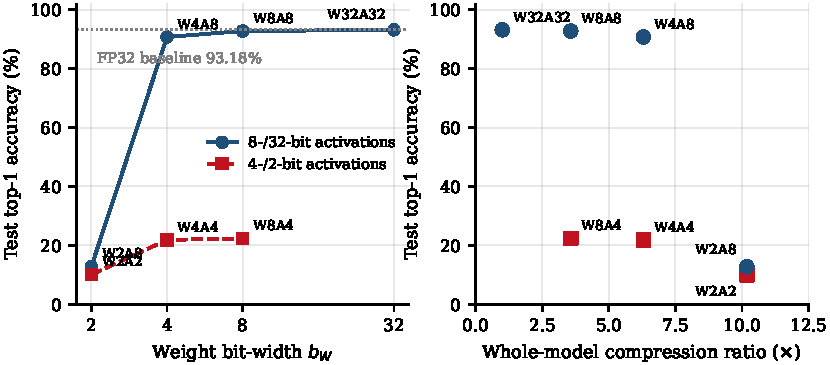
\includegraphics[width=\textwidth]{q2_uniform_sweep}
\caption{Uniform quantisation sweep. Left: test accuracy versus weight
bit-width, separated by activation width. Right: accuracy versus achieved
whole-model compression. Configurations with sub-8-bit activations sit below 25\%
irrespective of weight width.}
\label{fig:q2}
\end{figure}

%=============================================================================
\section{Q3 --- Sensitivity-Guided Mixed Precision}
\label{sec:q3}
%=============================================================================

\subsection{Layer Sensitivity}
Uniform allocation implicitly assumes that every layer tolerates quantisation
equally. HAWQ-V2~\cite{dong2020hawqv2} replaces that assumption with a
second-order criterion: a layer whose loss surface is sharply curved in its own
weights suffers more from a given perturbation than a flat one. For layer $l$
with $n_l$ weights and Hessian block $H_l$, the sensitivity score combines
average curvature with the perturbation that low-bit quantisation would actually
inflict,
\begin{equation}
\Omega_l = \left|\frac{\operatorname{Tr}(H_l)}{n_l}\right| \cdot
\bigl\| W_l - Q_4(W_l) \bigr\|_2^2 ,
\label{eq:omega}
\end{equation}
where $Q_4(\cdot)$ is the 4-bit quantiser of
Eqs.~\eqref{eq:scale}--\eqref{eq:quant}.

The Hessian trace is estimated with Hutchinson's
method~\cite{hutchinson1989stochastic}: for a Rademacher random vector $v$,
$\mathbb{E}[v^\top H v] = \operatorname{Tr}(H)$, and each Hessian-vector product
is obtained by double backpropagation through the loss. Estimates use 8 batches
$\times$ 8 probes for each of the 53 Conv/Linear layers. The absolute value in
Eq.~\eqref{eq:omega} is deliberate: the trained model sits near but not exactly at
a minimum, so a few layers return small negative trace estimates, and using the
signed value would rank those layers as the safest to compress, inverting the
intended ordering.

\subsection{Sensitive Layers}
Figure~\ref{fig:sens} ranks the twenty most sensitive layers. Sensitivity is
concentrated in the early stages of the network: the seven highest-scoring
layers are \texttt{features.1.conv.0.0}, \texttt{features.2.conv.1.0},
\texttt{features.2.conv.2}, \texttt{features.4.conv.2},
\texttt{features.1.conv.1}, \texttt{features.7.conv.2} and the stem
\texttt{features.0.0}. Two properties explain the concentration: early layers hold
few weights per output channel, so a coarse grid has little to average over and the
perturbation $\|W_l - Q_4(W_l)\|_2^2$ is larger, and they feed every subsequent
stage, so their error propagates through the full depth of the network. Later
stages, which hold most of the parameters, score low and are the ones that can be
pushed to 4 bits cheaply.

\begin{figure}[htbp]
\centering
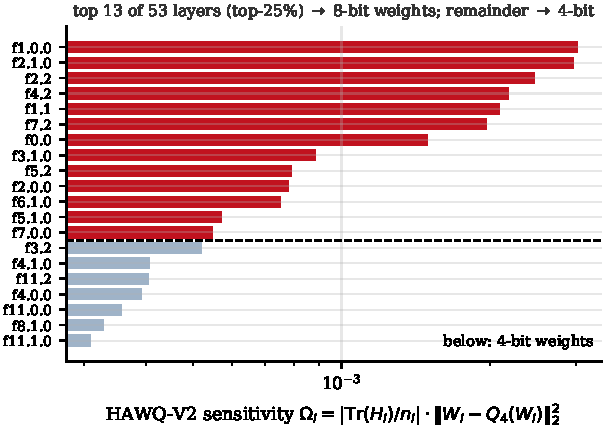
\includegraphics[width=0.74\textwidth]{hawq_sensitivity}
\caption{The twenty most sensitive of the 53 Conv/Linear layers, ranked by the
HAWQ-V2 score of Eq.~\eqref{eq:omega} on a logarithmic scale (layer names
abbreviated, \texttt{f}~$=$~\texttt{features}). The thirteen layers above the
dashed line form the top-25\% set retained at 8-bit weights.}
\label{fig:sens}
\end{figure}

\subsection{Mixed-Precision Results}
Layers are sorted by $\Omega_l$ and the top fraction retains 8-bit weights while
the remainder drops to 4 bits, with activations held at 8 bits.
Table~\ref{tab:mixed} reports the resulting sweep alongside the uniform
baselines, and Figure~\ref{fig:wandb} shows the corresponding Weights \& Biases
parallel-coordinates panel over weight width, activation width, compression
ratio, model size and accuracy. The runs were logged offline, so the figure is
the exported panel rather than a live dashboard.

Two comparisons carry the result. Against uniform 4-bit weights,
\texttt{hawq\_w8-4\_top25\_a8} gains $1.53$\,pt (92.28\% versus 90.75\%) at a
comparable compression ratio. Against uniform 8-bit weights,
\texttt{hawq\_w8-4\_top75\_a8} is simultaneously more accurate (92.94\% versus
92.78\%) and more compressed ($4.14\times$ versus $3.74\times$), so the ranking is
identifying genuinely different layer requirements rather than trading accuracy
for size along a fixed curve.

\TableMixed

\begin{figure}[htbp]
\centering
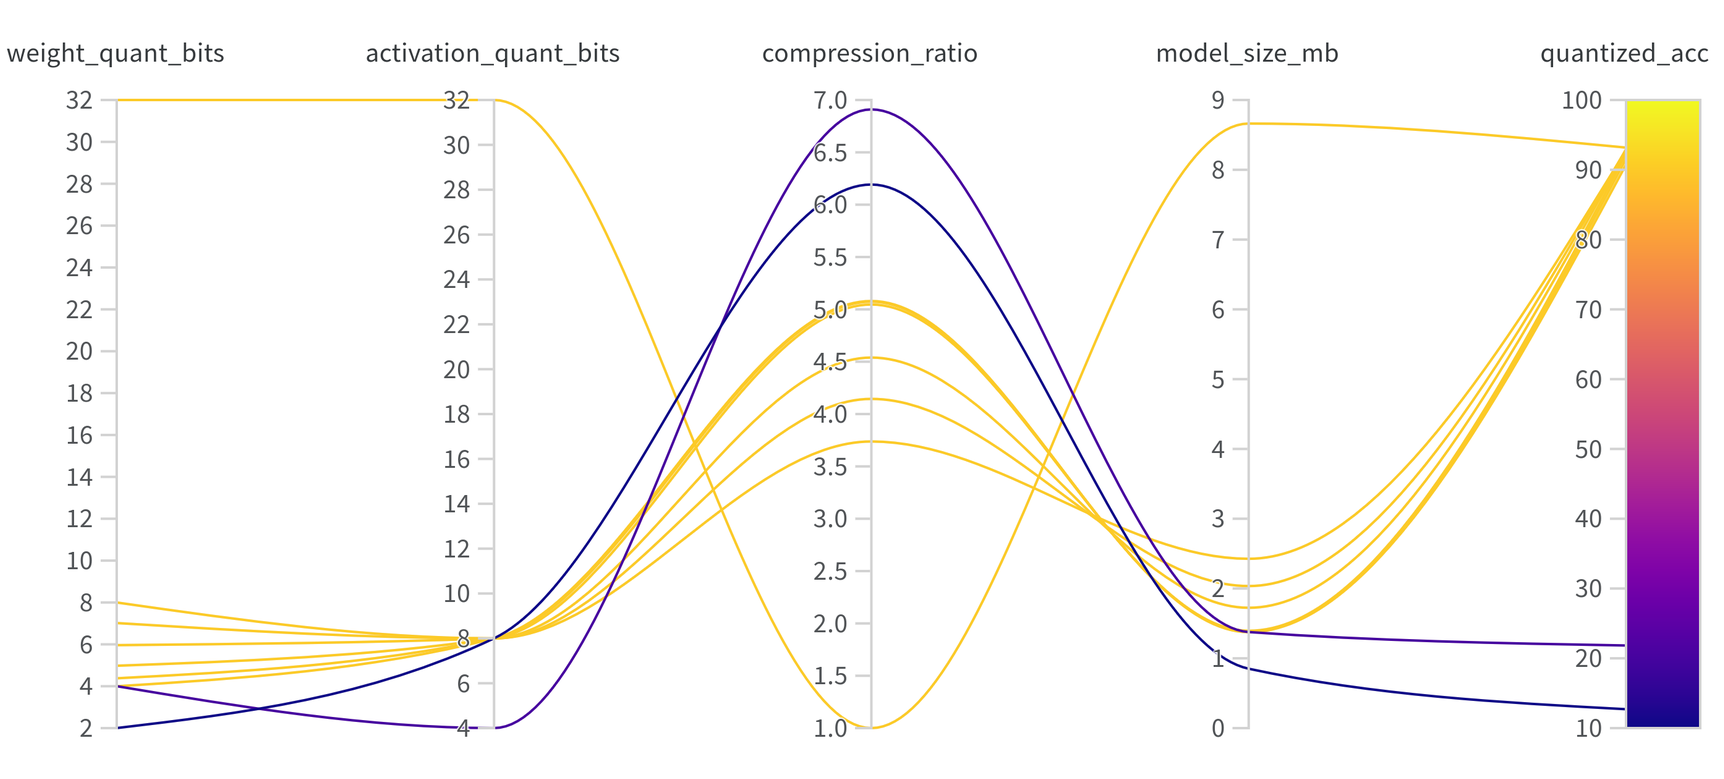
\includegraphics[width=\textwidth]{wandb_parallel_coordinates}
\caption{Weights \& Biases parallel-coordinates panel over the configurations of
Table~\ref{tab:mixed}, with axes for weight bit-width, activation bit-width,
compression ratio, model size and quantised accuracy. Each polyline is one run,
coloured by accuracy; runs were logged in offline mode.}
\label{fig:wandb}
\end{figure}

\subsection{Selected Configuration}
The selected configuration is \texttt{hawq\_w8-4\_top25\_a8}. The 13 most
sensitive of the 53 Conv/Linear layers retain 8-bit weights, the remaining 40 use
4-bit weights, giving an average weight width of 4.07 bits, and all quantised
activation inputs stay at 8 bits.

It sits at the knee of the accuracy/compression tradeoff: it reaches 92.28\% top-1,
$0.90$\,pt below the FP32 baseline, and improves on uniform W4A8 by $1.53$\,pt at
approximately the same model size (1.395 MB versus 1.376 MB). Configurations that
score higher cost substantially more memory for at most $0.7$\,pt, while everything
more compressed degrades sharply.

%=============================================================================
\section{Q4 --- Discussion}
%=============================================================================

\subsection{Weight versus Activation Precision}
The two sides of the network behave asymmetrically. Reducing weights to 4 bits
while holding activations at 8 costs $2.43$\,pt (W4A8, 90.75\%); reducing
activations to 4 bits while holding weights at 8 costs more than 70\,pt (W8A4,
22.36\%). Because weight width is identical between W8A8 and W8A4, the collapse
isolates cleanly to the activation path.

This asymmetry is a property of the calibration implemented here, not a general
statement about low-bit activations. Scales are set per tensor from the maximum
absolute value observed over the calibration set, so a single outlier fixes the
grid for the whole tensor and the sixteen levels available at 4 bits are spread
across the full observed range; the resulting error is then applied at each of the
53 quantised inputs. Alternative activation schemes --- percentile or MSE-optimal clipping, finer
granularity, or quantisation-aware fine-tuning --- were not evaluated here.

\subsection{Effect of Sensitivity-Guided Allocation}
Non-uniform allocation is worth more than the equivalent uniform budget. At
essentially the same size, \texttt{hawq\_w8-4\_top25\_a8} reaches 92.28\% against
90.75\% for \texttt{uniform\_w4a8}, a gain of $1.53$\,pt obtained purely by moving
thirteen layers back to 8 bits. At the other end of the range, \texttt{hawq\_w8-4\_top75\_a8} reaches 92.94\% against
92.78\% for \texttt{uniform\_w8a8}, beating uniform 8-bit on accuracy while also
being smaller. Spending the precision budget where curvature is highest therefore
dominates spending it evenly.

\subsection{Final Storage Accounting}
\label{sec:storage}
Table~\ref{tab:final} audits the selected configuration. The packed weights
occupy 1.069 MB against 8.402 MB in FP32, a $7.86\times$ reduction. Activation
memory, measured as the sum of the input tensors of the 53 quantised operators
for a single image, falls from 6.194 MB to 1.549 MB, exactly $4.00\times$ at 8
bits. The complete model is 1.395 MB against 8.662 MB, a whole-model ratio of
$6.21\times$.

The whole-model ratio is lower than the weight ratio because it charges for
everything the model needs in order to run. Scale metadata contributes
68{,}476\,B --- one FP32 scale per output channel across the quantised layers plus
one per layer input --- and the retained FP32 BatchNorm and bias tensors
contribute 272{,}936\,B. Together these are about a quarter of the compressed
model, and neither shrinks when the weight width is reduced further.

\TableFinal

\subsection{Overall Interpretation}
Sensitivity-guided mixed precision yields a better accuracy/compression tradeoff
than uniform allocation because it retains higher precision only for the layers
genuinely sensitive to quantisation, and those layers hold a small fraction of the
parameters; uniform allocation must pay for precision across the entire network,
including the late stages that tolerate 4 bits without measurable loss.

The accounting adds a systems-level qualification to that result. As the
quantised weight payload shrinks, the fixed costs --- scale metadata and the
tensors deliberately retained in FP32 --- come to dominate the model size. They
are already 23.4\% of the compressed model at 1.395 MB, which is why the
whole-model compression curve flattens well before the weight-side curve does,
and why further reductions in weight width would return progressively less. Any
realistic model-size claim must include them.

%=============================================================================
\section{Conclusion}
%=============================================================================
A CIFAR-adapted MobileNet-v2 trained from scratch reaches 93.18\% top-1 on
CIFAR-10. Uniform quantisation of that baseline reveals a strong asymmetry
between the two precision budgets: 4-bit weights with 8-bit activations remain
usable at 90.75\%, whereas sub-8-bit activations fail under the max-absolute
per-tensor calibration implemented here, collapsing to 22.36\% even with 8-bit
weights retained. Ranking the 53 Conv/Linear layers by a HAWQ-V2-inspired
sensitivity score improves the allocation of the weight budget, recovering
accuracy at unchanged size.

The selected configuration, \texttt{hawq\_w8-4\_top25\_a8}, assigns 8-bit weights
to 13 layers and 4-bit weights to the remaining 40, with all quantised
activations at 8 bits. It attains 92.28\% top-1 accuracy at a final model size of
1.395 MB, corresponding to $7.86\times$ weight compression, $4.00\times$
activation compression and $6.21\times$ whole-model compression including all
quantisation metadata and retained FP32 tensors.

{\footnotesize
\bibliographystyle{plain}
\bibliography{references}}

\end{document}
